\documentclass[12pt,a4paper]{report}
\usepackage[top=1.2in,right=1.2in,left=1.2in,bottom=1in]{geometry}
\usepackage[english,slovene]{babel}
\usepackage[cp1250]{inputenc}
\usepackage[T1]{fontenc}
\usepackage{color}
\usepackage[pdftex]{graphicx}
\usepackage{exscale}
\usepackage{amsmath}
\usepackage{amssymb}
\usepackage[pdftex,bookmarks,colorlinks]{hyperref}
\usepackage{verbatim}
\usepackage[pdftex]{graphicx}
\usepackage{float}		% floating pictures and tables
\usepackage{multirow}	% multirow table input
\usepackage{listings}	% for input of programming code
\usepackage{titlesec}	% for alternative title settings
\usepackage{upgreek}	% for upright greek letters (\upalpha, \upbeta,...)
\usepackage[nomessages]{fp}		% for arithmetics of high precision real point numbers
\usepackage{enumitem}	% for setting spacings in itemize
\usepackage{booktabs}	% nicer tables
\usepackage{epstopdf}	% transforms all eps plots to pdf
\usepackage[titletoc]{appendix}	% for setting appendix chapter title options
\usepackage{url}	% for url links
\usepackage{subfigure} % for making subfigures
\usepackage{verbatim}
\usepackage[]{units}
\usepackage[table]{xcolor}
\usepackage{lineno}
\hypersetup{colorlinks,%
	citecolor=black,%
	filecolor=black,%
	linkcolor=black,%
	urlcolor=blue,%
	pdftex}

%\titleformat{\chapter}[hang]{\huge\bf}{\thechapter}{1em}{}
%\titlespacing{\chapter}{0pt}{0pt}{1cm}
\titleformat{\chapter}[hang]{\normalfont\bf}{}{12pt}{\huge}
\titlespacing{\chapter}{0pt}{0pt}{1cm}
\titleformat{\section}[hang]{\normalfont\bf}{}{12pt}{\Large\thesection\enspace}
\titleformat{\subsection}[hang]{\normalfont\bf}{}{12pt}{\large\thesubsection\enspace}

% definitions of commands and environments
\newcommand{\diff}{\operatorname{d}\!}	% operator d for integration or differentiation
\newcommand{\pdiff}{\partial}	% operator for partial differentiation
\newcommand{\iu}{{i\mkern1mu}}	% imaginary unit i
\newcommand{\me}{\, \mathrm{e}}	% natural exponential e
\newcommand{\mytilde}{\raise.17ex\hbox{$\scriptstyle\mathtt{\sim}$}}		% tilde sign, denoting similarity
\newcommand{\quotes}[1]{``#1''}	% quotes
\newcommand*\rfrac[2]{{}^{#1}\!/_{#2}}	% inline fractions

%\makeatletter
%\newcommand{\customlabel}[2]{%	creates custom labels (1st argument is reference name, 2nd is what is displayed
%   \protected@write \@auxout {}{\string \newlabel {#1}{{#2}{\thepage}{#2}{#1}{}} }%
%   \hypertarget{#1}{}%#2}
%}
%\makeatother

\newcommand{\ra}[1]{\renewcommand{\arraystretch}{#1}}	% horizontally stretches tables

\definecolor{lightyellow}{RGB}{255,255,153}	% defines a new color (light yellow)
\definecolor{lighteryellow}{RGB}{255,255,204}	% defines a new color (even lighter yellow)
\definecolor{white}{RGB}{255,255,255}	% defines a new color (white)

%\setlist[itemize]{itemsep=1pt, topsep=3pt}	% sets global spacings for lists
\setlist[itemize]{itemsep=1pt, topsep=2pt, after=\newline}	% sets global spacings for lists

\definecolor{light-gold}{cmyk}{0,0.05,0.2,0}

\lstnewenvironment{code}{%
  \lstset{backgroundcolor=\color{white},
  frame = single,
  framerule = 0pt,
  basicstyle = \ttfamily,
  basicstyle=\footnotesize}}{}

\begin{document}

\selectlanguage{english}

\chapter{Usage instructions}
The following instructions go over usage instructions for the auger-analysis program. They also explain individual parts of the source code and give instructions for adding new options to the program.

\section{The graphical interface}
The GUI of the program for ADST version \texttt{XrYpZ} is executed with:
\begin{verbatim}
   ./start.sh vXrYpZ
\end{verbatim}
Note that standard output to the terminal might slow down the program considerably. It is thus advised to save the standard output into a file with:
\begin{verbatim}
   ./start.sh vXrYpZ > results/printout.txt
\end{verbatim}
This opens the initial graphical interface of the program:\\
\centerline{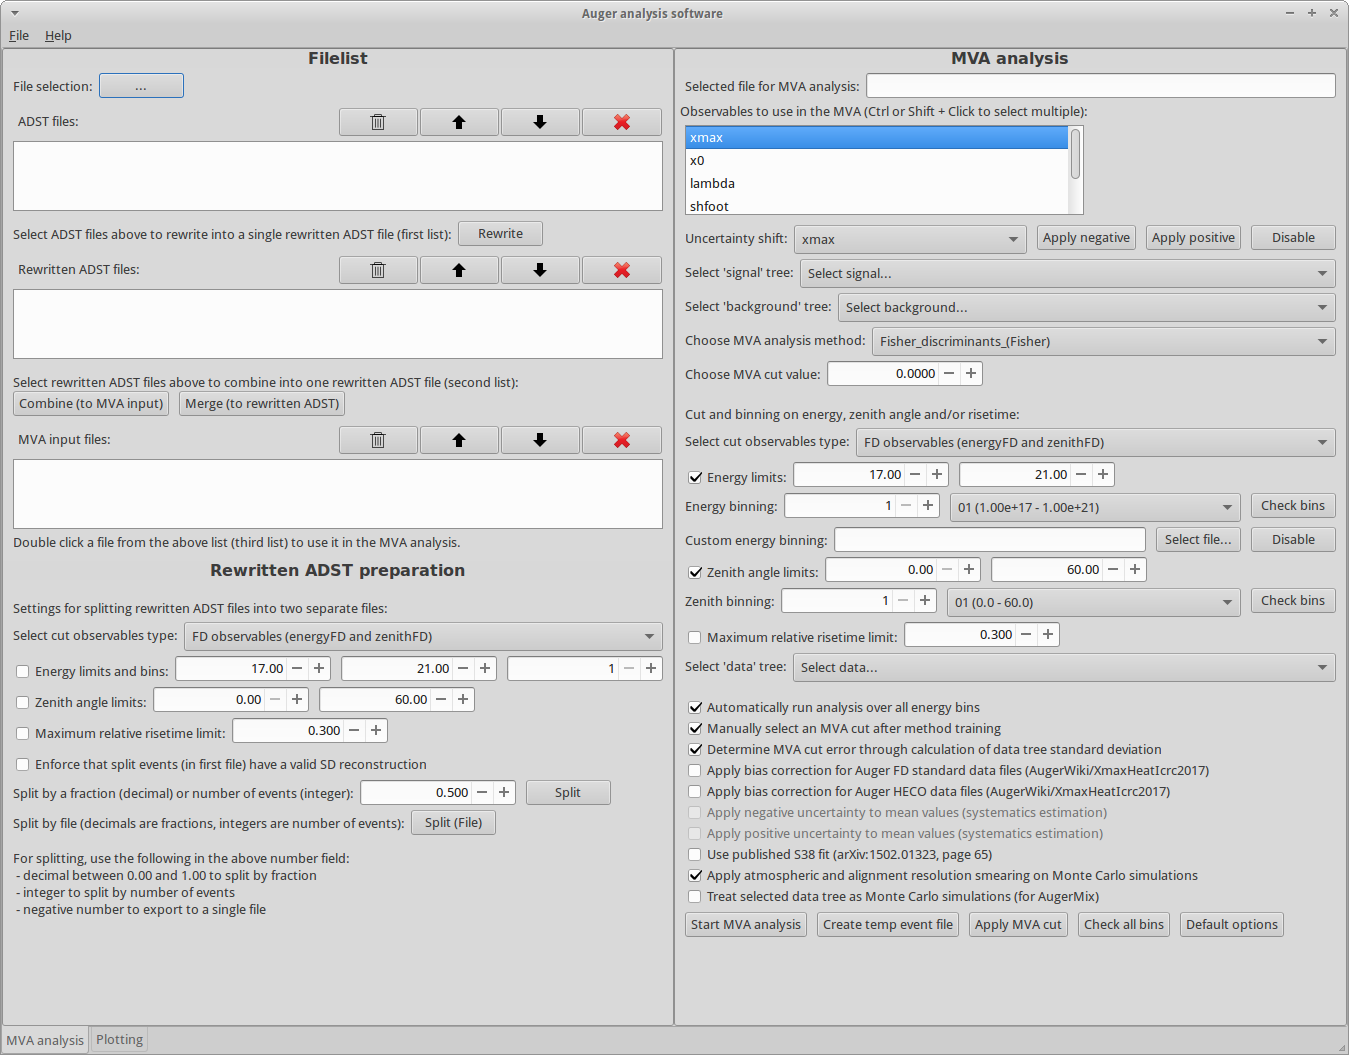
\includegraphics[width=0.999\textwidth]{figures/software_screenshot_1.png}}\\

Moving to the \texttt{Plotting} tab in the bottom left, we get to the plotting part of the program:\\
\centerline{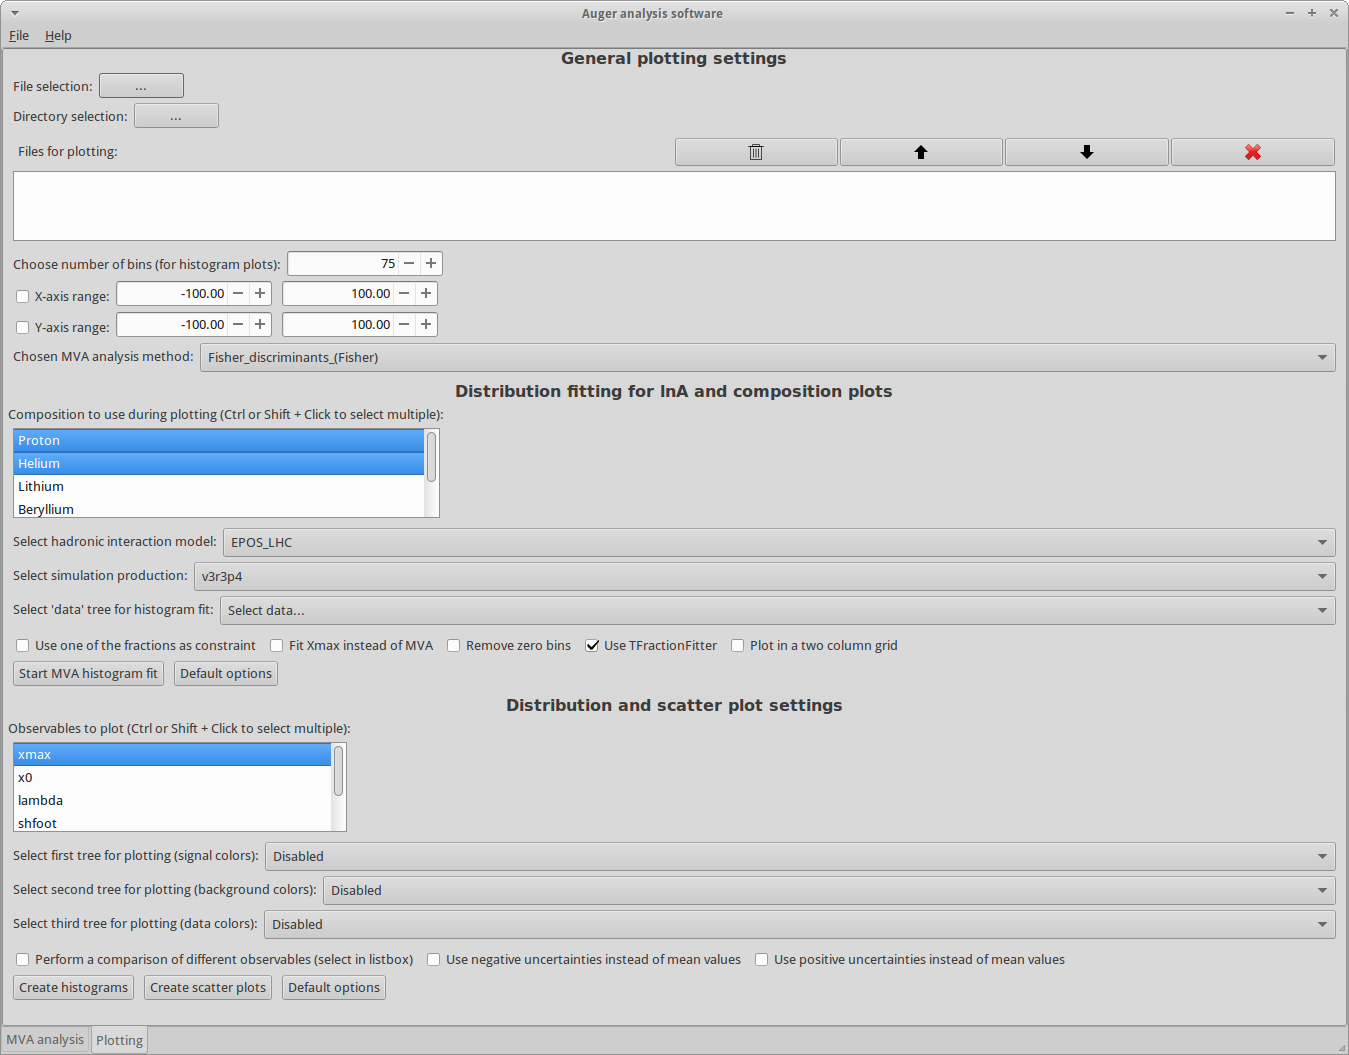
\includegraphics[width=0.999\textwidth]{figures/software_screenshot_2.png}}\\

%\chapter{Installation instructions}
%The following instructions go over the complete installation procedure for compiling the auger-analysis program.
%
%\section{Folder structure}
%The folder structure of the auger-analysis program is as follows. The base non-compiled version of the program has:
%\begin{itemize}
%\item[--] \texttt{configure}: Script for configuring the compilation and running the installation.
%\item[--] \texttt{doc}: Documentation for the program. Installation and usage instructions.
%\item[--] \texttt{include}: Folder containing all header files.
%\item[--] \texttt{input}: Folder containing input files that are needed by some program options.
%\item[--] \texttt{layout}: Folder containing program GUI layout instructions.
%\item[--] \texttt{set\_environment.sh}: Script for setting up environmental variables.
%\item[--] \texttt{setup}: Folder containing additional setup files needed in the configuration.
%\item[--] \texttt{src}: Folder containing all source code files.
%\end{itemize}
%The fully compiled version of the program also has:
%\begin{itemize}
%\item[--] \texttt{bin}: Folder containing all executables.
%\item[--] \texttt{lib}: Folder containing all created libraries.
%\item[--] \texttt{results}: Default folder for saving analysis results. When cleaning the installation, this folder remains unchanged.
%\item[--] \texttt{start.sh}: Script for running the GUI or batch version of the program.
%\end{itemize}
%
%\section{Installation prerequisites}
%For this software to work correctly, ROOT \cite{root}, wxWidgets \cite{wxWidgets} and their prerequisites need to be installed on the system. The following packages are essential on a clean installation of Linux, before either ROOT or wxWidgets can be installed. General purpose prerequisites are:
%\begin{verbatim}
%   sudo apt-get install git patch build-essential cmake gcc g++ \
%     gfortran python doxygen python-dev wget
%\end{verbatim}
%ROOT software prerequisites are:
%\begin{verbatim}
%   sudo apt-get install libx11-dev libxpm-dev libxft-dev \
%     libxext-dev libpng libjpeg libgsl0-dev libfftw3-dev \
%     libmysqlclient-dev libxml2-dev
%\end{verbatim}
%wxWidgets software prerequisites are:
%\begin{verbatim}
%   sudo apt-get install libgtk2.0-dev libc++1
%\end{verbatim}
%These packages, ROOT, wxWidgets and the auger-analysis program have been tested on Linux distributions Mint 18.2 (sonya) and Ubuntu 14.04 (trusty) and work as expected.
%
%\section{Installing ROOT}
%ROOT is a data analysis framework able to handle python or C/C++ code integration. The complete instructions are available on the software page at \cite{root}. We assume here, that \texttt{\$ROOTSOURCE} is the location of the downloaded source files and \texttt{\$ROOTINSTALL} is the location of the ROOT installation.\\
%ROOT versions 5.XX.YY are installed as (installation of version 5.34.36 or higher is suggested):
%\begin{verbatim}
%   cd $ROOTSOURCE
%   wget -nc https://root.cern.ch/download/root_v5.XX.YY.source.tar.gz
%   tar -zxf root_v5.XX.YY.source.tar.gz
%   mv ./root $ROOTINSTALL/root-5.XX.YY
%   cd $ROOTINSTALL/root-5.XX.YY
%   ./configure --enable-mysql --enable-python --enable-minuit2 \
%     --enable-roofit --enable-tmva --enable-xml \
%     --enable-builtin-freetype
%   make
%\end{verbatim}
%ROOT versions 6.XX.YY are installed as:
%\begin{verbatim}
%   cd $ROOTSOURCE
%   wget -nc https://root.cern.ch/download/root_v6.XX.YY.source.tar.gz
%   tar -zxf root_v6.XX.YY.source.tar.gz
%   cd $ROOTSOURCE/root-6.XX.YY
%   mkdir ./builddir
%   cd ./builddir
%   cmake ../ -DCMAKE_INSTALL_PREFIX=$ROOTINSTALL/root-6.XX.YY \
%     -Dmysql=ON -Dpython=ON -Dminuit2=ON -Droofit=ON -Dtmva=ON \
%     -Dxml=ON -Dbuiltin-freetype=ON
%   cmake --build .
%   cmake --build . --target install
%\end{verbatim}
%In order to setup their environmental variables once installed, run one of the following commands:
%\begin{verbatim}
%   source $ROOTINSTALL/root-5.XX.YY/bin/thisroot.sh
%   source $ROOTINSTALL/root-6.XX.YY/bin/thisroot.sh
%\end{verbatim}
%The following command should now return the correct version of ROOT:
%\begin{verbatim}
%   root-config --version
%\end{verbatim}
%
%\section{Installing wxWidgets}
%wxWidgets is a cross-platform GUI library used for the graphical user interface of the auger-analysis program. The complete instructions are available on the software page at \cite{wxWidgets}. We assume here, that \texttt{\$WXSOURCE} is the location of the downloaded source files and \texttt{\$WXINSTALL} is the location of its installation.\\
%wxWidgets version X.Y.Z is installed as (installation of version 3.0.3 or higher is suggested):
%\begin{verbatim}
%   cd $WXSOURCE
%   wget -nc https://github.com/wxWidgets/wxWidgets/releases/\
%     download/vX.Y.Z/wxWidgets-X.Y.Z.tar.bz2
%   tar -jxf wxWidgets-X.Y.Z.tar.bz2
%   cd $WXSOURCE/wxWidgets-X.Y.Z
%   mkdir ./gtk-build
%   cd ./gtk-build
%   ./configure --enable-unicode --enable-debug --prefix=$WXINSTALL
%   make
%   make install
%\end{verbatim}
%For wxWidgets to be correctly recognized, add the following environmental variables (preferrably in the \texttt{~/.bashrc} script):
%\begin{verbatim}
%   export WXLIN=$WXINSTALL/wxWidgets-X.Y.Z
%   export PATH=$WXLIN/bin:$PATH
%   export LD_LIBRARY_PATH=$WXLIN/lib:$LD_LIBRARY_PATH
%\end{verbatim}
%The following command should now return the correct version of wxWidgets:
%\begin{verbatim}
%   wx-config --version
%\end{verbatim}
%
%\section{Installing ADST reader}
%The ADST reader is part of the Offline software developed by the Pierre Auger Observatory \cite{offline}. A handful of versions have been included with this software and are automatically installed, when needed. See section \ref{sec:install} for installation of the auger-analysis program.\\
%If a new version of the ADST reader is needed, add its tar-ball into folder \texttt{setup} and name it \texttt{ADST\_vXrYpZ.tar.gz}, where \texttt{XrYpZ} denotes the version. The configure script will then automatically recognize that there is an additional version of the ADST reader available.
%
%\section{Installing external TMVA}
%TMVA is the multivariate analysis package for ROOT \cite{tmva}. New versions have been implemented directly into ROOT versions 6.XX.YY, while ROOT 5.XX.YY can use an external version of TMVA. For this purpose, the TMVA version 4.2.0 has been included with this software and is automatically installed. See section \ref{sec:install} for installation of the auger-analysis program.
%
%\section{Installation of the auger-analysis program} \label{sec:install}
%Once the above prerequesites and installations have been satisfied, it is now possible to install the auger-analysis program. The complete program is compiled and installed through a single call of the configure script:
%\begin{verbatim}
%   ./configure vXrYpZ
%\end{verbatim}
%Here, the program is installed using ADST version \texttt{XrYpZ}, but other options can simply be checked by running \texttt{./configure} or \texttt{./configure help}.

\pagebreak
\begin{thebibliography}{50} \addcontentsline{toc}{section}{Bibliography}
\raggedright
\bibitem{root} ROOT data analysis framework, \href{https://root.cern.ch}{\texttt{https://root.cern.ch}}.
\bibitem{wxWidgets} wxWidgets cross-platform GUI library, \href{https://www.wxwidgets.org}{\texttt{https://www.wxwidgets.org}}.
\bibitem{offline} S. Argiro, \emph{et al.}, \emph{The Offline Software Framework of the Pierre Auger Observatory}, \href{http://arxiv.org/pdf/0707.1652v1.pdf}{\texttt{arXiv:0707.1652}} (1998).
\bibitem{tmva} Toolkit for Multivariate Analysis (TMVA), \href{http://tmva.sourceforge.net}{\texttt{http://tmva.sourceforge.net}}.
\end{thebibliography}

\end{document}
